\documentclass[tikz,border=5pt]{standalone}
\usepackage[T1]{fontenc}
\usepackage{lmodern,amsmath,amssymb}
\usetikzlibrary{arrows.meta,calc,positioning,fit,backgrounds,shapes.geometric,matrix,decorations.pathreplacing,patterns}
\definecolor{ink}{gray}{0.08}
\definecolor{wash}{gray}{0.965}
\definecolor{soft}{gray}{0.45}
\tikzset{box/.style={draw=ink,line width=.65pt,fill=white,align=center,inner sep=4pt,outer sep=0pt,font=\small},flow/.style={draw=ink,line width=.65pt,-{Latex[length=1.8mm,width=1.3mm]},rounded corners=2pt},annotation/.style={font=\scriptsize,text=soft,align=center},groupbox/.style={draw=soft,dashed,line width=.45pt,fill=wash}}
\begin{document}
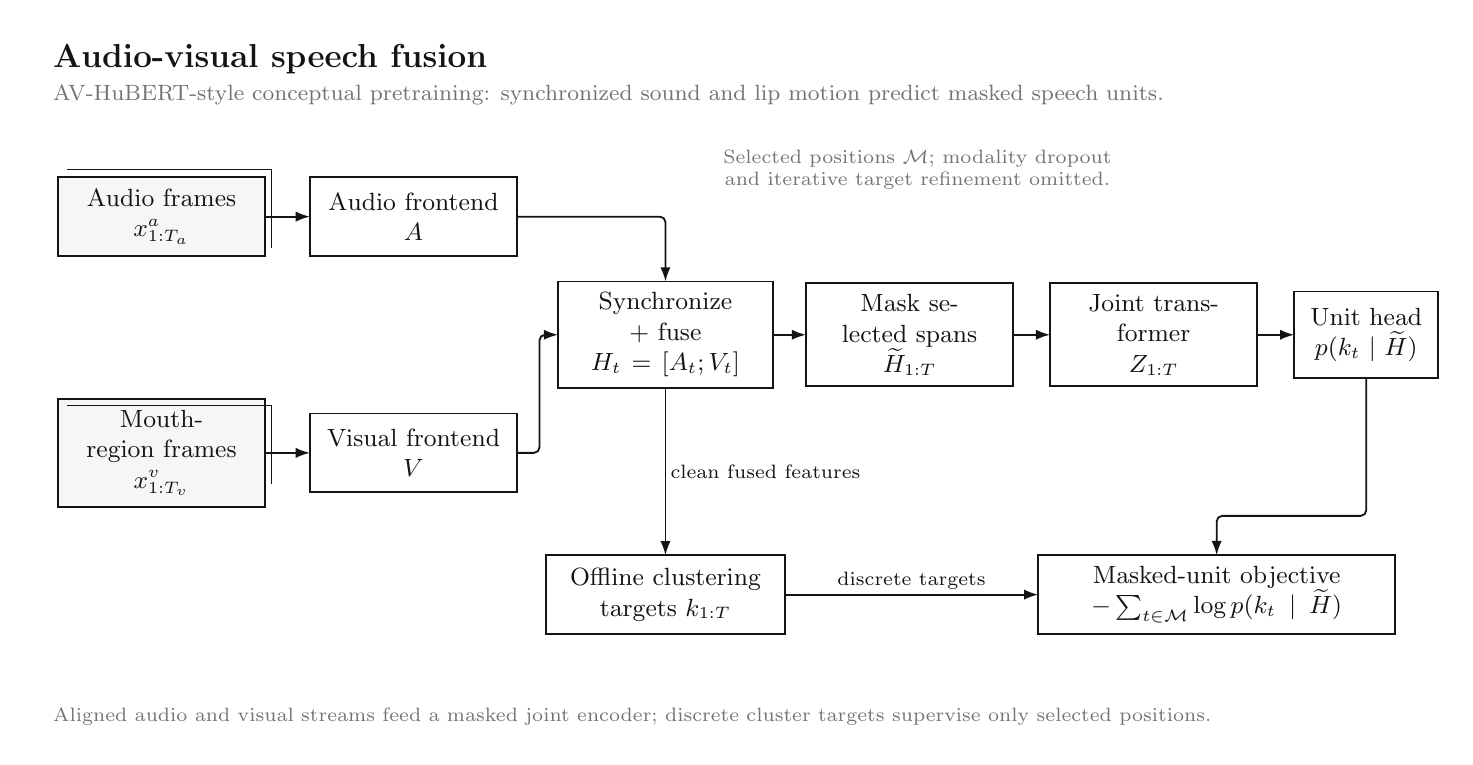
\begin{tikzpicture}[x=1cm,y=-1cm,font=\rmfamily,text=ink]

\path[use as bounding box] (0,0) rectangle (18,9);
\node[anchor=west,font=\large\bfseries] at (.2,.4) {Audio-visual speech fusion};
\node[anchor=west,font=\footnotesize,text=soft] at (.2,.85) {AV-HuBERT-style conceptual pretraining: synchronized sound and lip motion predict masked speech units.};
\begin{pgfonlayer}{background}
\end{pgfonlayer}
\node[box,fill=wash,minimum width=2.6cm,minimum height=1cm,text width=2.35cm] (audio) at (1.7,2.4) {Audio frames\\$x^a_{1:T_a}$};
\draw[ink,line width=.4pt] (0.4999999999999999,1.7999999999999998) -- (3.1,1.7999999999999998) -- (3.1,2.8);
\node[box,fill=wash,minimum width=2.6cm,minimum height=1cm,text width=2.35cm] (video) at (1.7,5.4) {Mouth-region frames\\$x^v_{1:T_v}$};
\draw[ink,line width=.4pt] (0.4999999999999999,4.800000000000001) -- (3.1,4.800000000000001) -- (3.1,5.800000000000001);
\node[box,minimum width=2.6cm,minimum height=1cm,text width=2.35cm] (aenc) at (4.9,2.4) {Audio frontend\\$A$};
\node[box,minimum width=2.6cm,minimum height=1cm,text width=2.35cm] (venc) at (4.9,5.4) {Visual frontend\\$V$};
\node[box,minimum width=2.7cm,minimum height=1.2cm,text width=2.45cm] (align) at (8.1,3.9) {Synchronize + fuse\\$H_t=[A_t;V_t]$};
\node[box,minimum width=2.6cm,minimum height=1.1cm,text width=2.35cm] (mask) at (11.2,3.9) {Mask selected spans\\$\widetilde H_{1:T}$};
\node[box,minimum width=2.6cm,minimum height=1.1cm,text width=2.35cm] (joint) at (14.3,3.9) {Joint transformer\\$Z_{1:T}$};
\node[box,minimum width=1.8cm,minimum height=1.1cm,text width=1.55cm] (pred) at (17.0,3.9) {Unit head\\$p(k_t\mid\widetilde H)$};
\node[box,minimum width=3.0cm,minimum height=1.0cm,text width=2.75cm] (clusters) at (8.1,7.2) {Offline clustering\\targets $k_{1:T}$};
\node[box,minimum width=4.5cm,minimum height=1.0cm,text width=4.25cm] (loss) at (15.1,7.2) {Masked-unit objective\\$-\sum_{t\in\mathcal M}\log p(k_t\mid\widetilde H)$};
\begin{pgfonlayer}{background}
\draw[flow] (audio.east) -- (aenc.west);
\draw[flow] (video.east) -- (venc.west);
\draw[flow] (aenc.east) -- (8.1,2.4) -- (align.north);
\draw[flow] (venc.east) -- (6.5,5.4) -- (6.5,3.9) -- (align.west);
\draw[flow] (align.east) -- (mask.west);
\draw[flow] (mask.east) -- (joint.west);
\draw[flow] (joint.east) -- (pred.west);
\draw[flow] (align.south) -- (clusters.north) node[midway,right,fill=white,inner sep=1.5pt,font=\scriptsize] {clean fused features};
\draw[flow] (clusters.east) -- (loss.west) node[midway,above,fill=white,inner sep=1.5pt,font=\scriptsize] {discrete targets};
\draw[flow] (pred.south) -- (17.0,6.2) -- (15.1,6.2) -- (loss.north);
\end{pgfonlayer}
\node[annotation,text width=9.5cm] at (11.3,1.8) {Selected positions $\mathcal M$; modality dropout and iterative target refinement omitted.};
\node[anchor=west,align=left,font=\scriptsize,text=soft,text width=17.6cm] at (.2,8.75) {Aligned audio and visual streams feed a masked joint encoder; discrete cluster targets supervise only selected positions.};
\end{tikzpicture}
\end{document}
